\section{Lecture 11}

Thursday, October 16th 2025. I was gone this day, so I copied notes from J. Liang.

\begin{itemize}
    \item Dof
          \[ \chi^2(\theta) = (y- A \vec{\theta})^T V^{-1} (y - A \vec{\theta}) \]
    \item At $\hat{\theta}$, $\chi^2$ is minimized:
          \[ \pdv{\chi^2}{\theta}\bigg|_{\theta = \hat{\theta}} = 0 = F(\vec{y} | \vec{\theta}, \vec{x}) = \begin{matrix}
                  F(\vec{y} | \theta_1, \vec{x}) \\
                  F(\vec{y} | \theta_2, \vec{x}) \\
                  \vdots                         \\
                  F(\vec{y} | \theta_k, \vec{x})
              \end{matrix}\]
    \item i.e. linear fit $\vec{y} = A \vec{\theta}$, k-equations:
          \[ \hat{\theta} = (A^T V^{-1} A)^{-1} (A^T V^{-1}) \vec{y} \]
    \item Think about it like this: If I know n-k $y_i$'s, the remaining k $y_i$'s are fixed. Their relations might be not obvious and complex but they're fixed. This is just cause we have k-equations.

          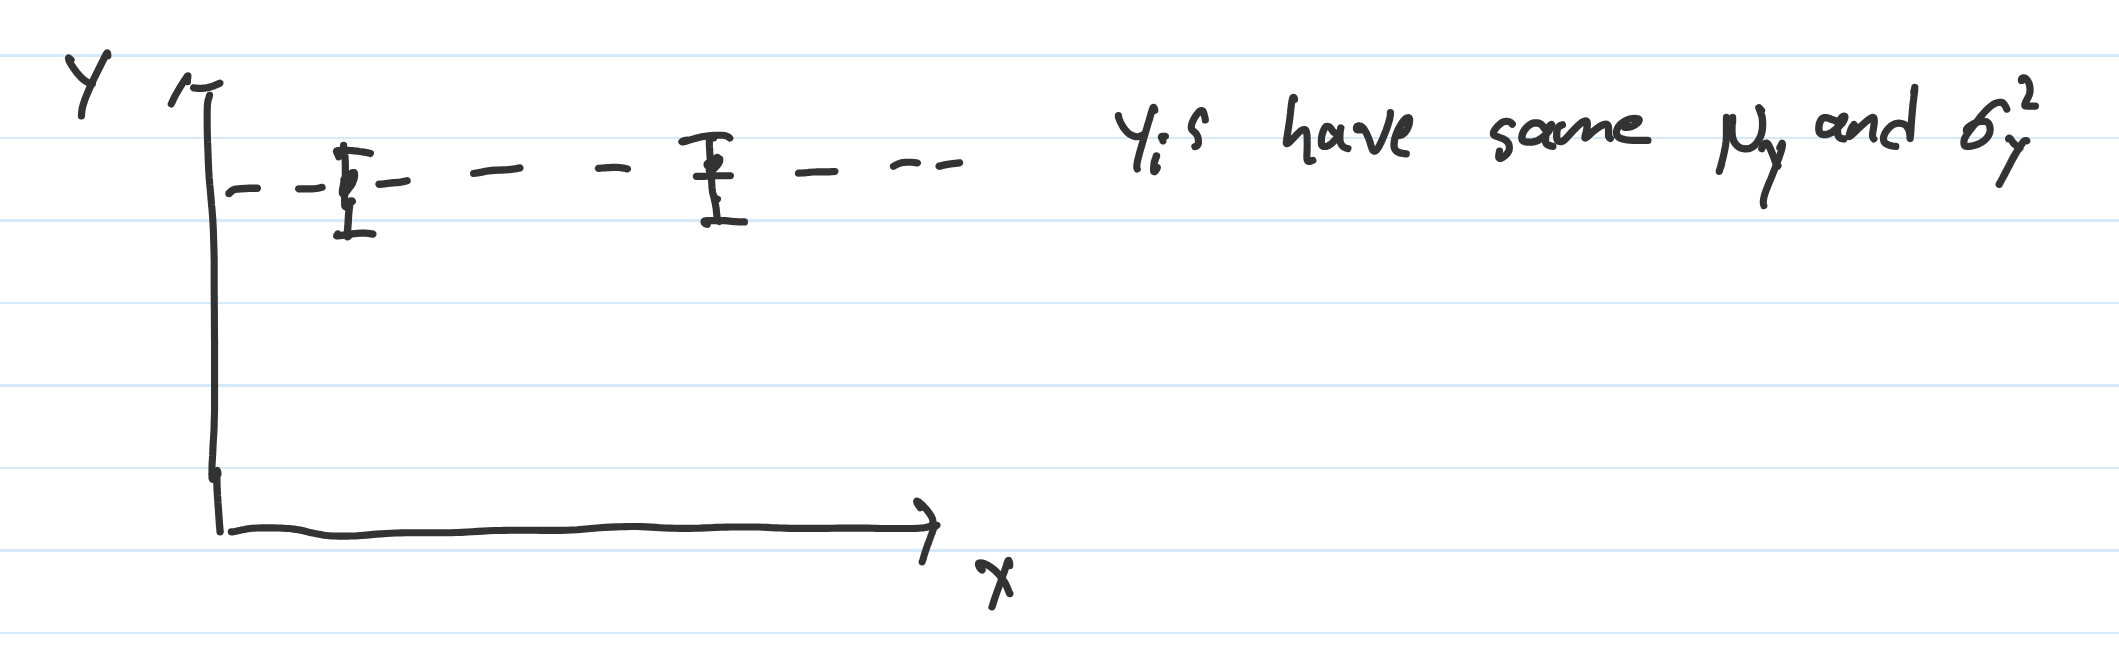
\includegraphics[width=0.8 \linewidth]{Images/lec11-chisqu-example.png}

          $y_i$'s have some $N_y$ and $\sigma_y^2$.
    \item Best estimator of true N is $\hat{y} = \frac{y_1+y_2}{2}$
          \[ \chi^2 = \left(\frac{y_1 - \hat{N}}{\sigma_y}\right)^2 + \left(\frac{y_2 - \hat{N}}{\sigma_y}\right)^2 \]
    \item Note:
          \[ y_1 - \hat{N} = \frac{1}{2} (y_1 - y_2)\]
          \[ y_2 - \hat{N} = \frac{1}{2} ( y_2- y_1)\]
    \item Where $z_1 = y_1 - y_2$, and $z_2 = y_2 - y_1$ such that $z_2 = - z_1$.
          \[ V(z_1, z_2) = \begin{pmatrix}
                  1  & -1 \\
                  -1 & 1
              \end{pmatrix} \]
    \item Determinant of V is 0, so not invertible.
    \item So basically we really only just have one independent variable.
    \item Residual: $ r_i = y_i - f_i(\vec{\theta})$
    \item When talking about goodness of fit, people usually divide y by dof so if $\chi^2/dof \approx 1$, it's a good fit.
    \item What about residuals?

          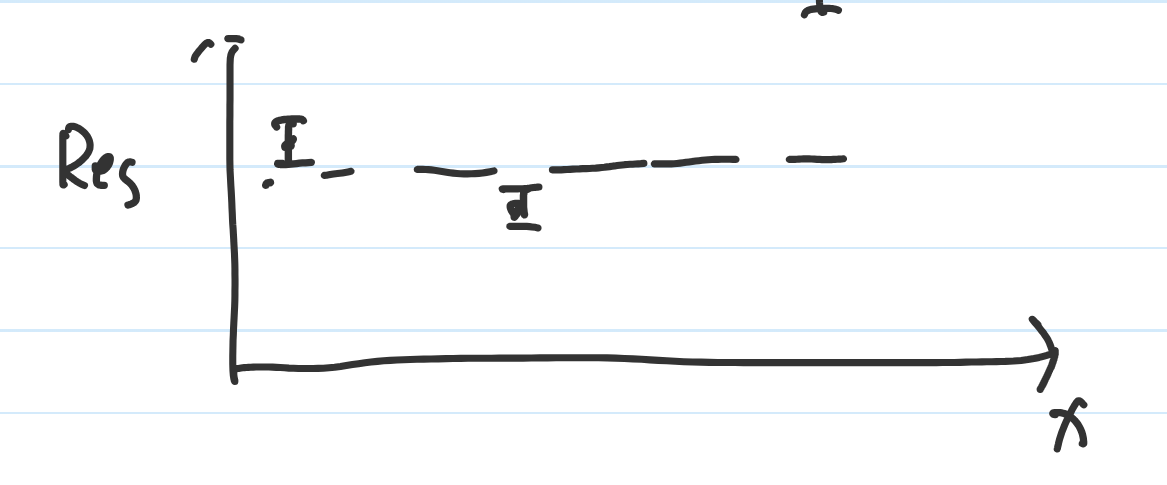
\includegraphics[width=0.5\linewidth]{Images/lec11-residual.png}

          Sometimes one weird data point can throw off the whole $\chi^2$, in weird ways. So gotta check residuals too.
    \item If residuals are randomly scattered around 0, it's a good fit.

          \divider
    \item We've been talking about estimators, but we want values of the params.
    \item Suppose we perform a fit on a param with the value a.
    \item From fitting we get diff estimator value from diff data sets.
          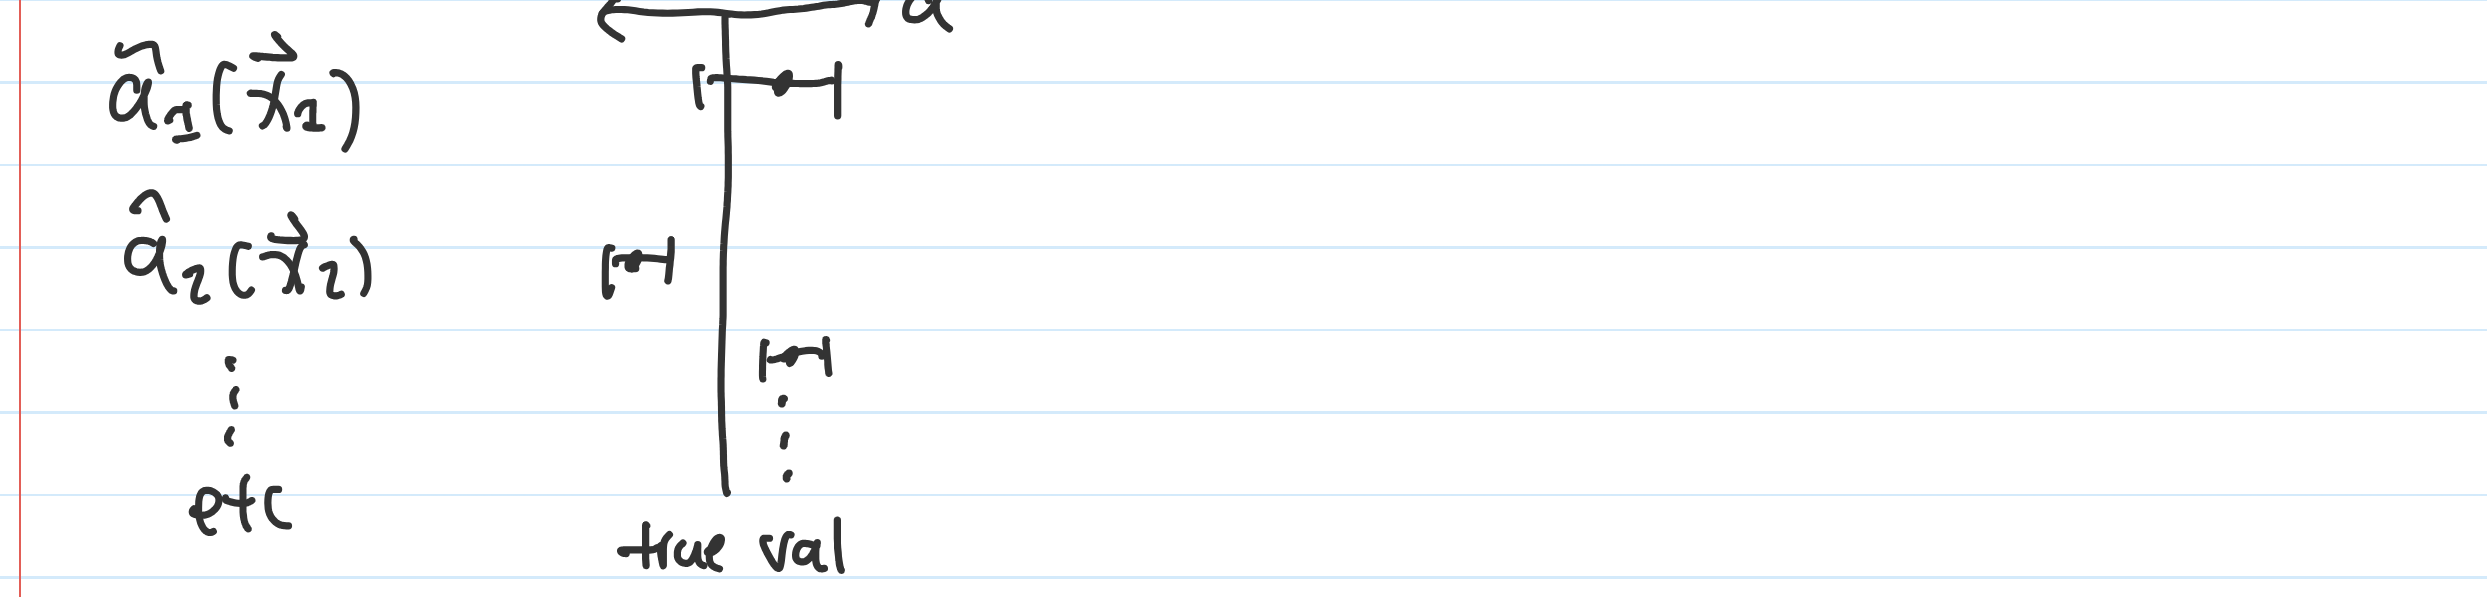
\includegraphics[width = 0.5 \linewidth]{Images/lec11-spread-est-vals.png}
    \item But they can be scattered all over the place.

          \divider
    \item Toy Monte Carlo:
          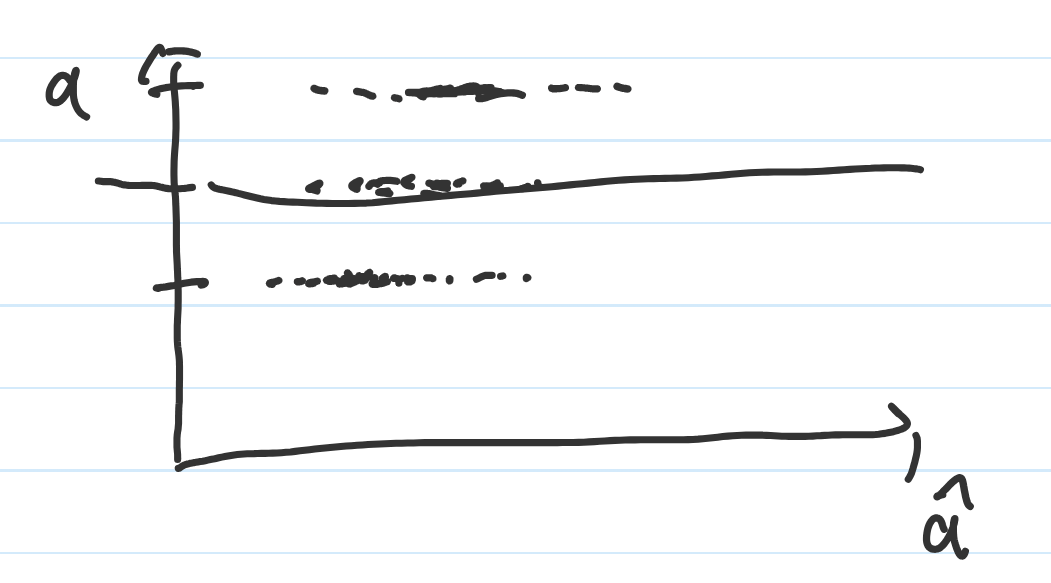
\includegraphics[width = 0.6\linewidth]{Images/lec11-toy-monte-carlo.png}
    \item Often model is too complicated to get analytic form of estimator distribution.
          \begin{enumerate}
              \item Pick an a
              \item Generate many data sets according to model with param a
              \item For each data set, compute estimator $\hat{a}$
              \item Plot histogram of $\hat{a}$
              \item Repeat step 2 n times
              \item Repeat step 1 m times
          \end{enumerate}
    \item I can do for each a value, 5\% vs 90\% vs 5\%. \\
          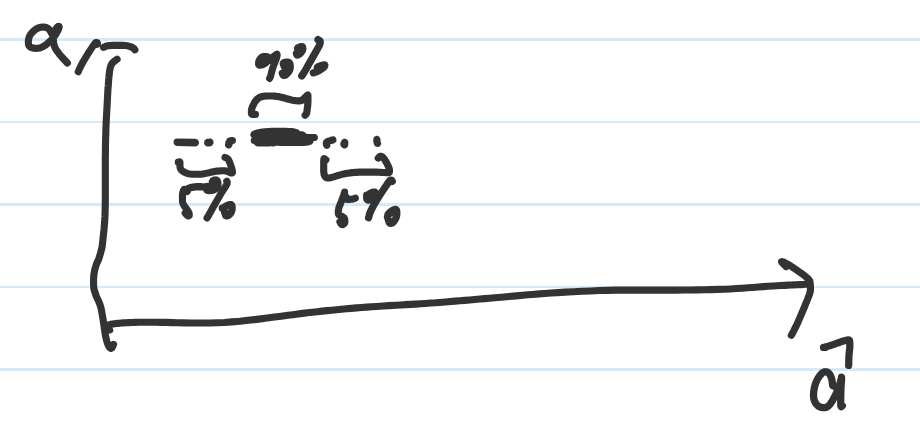
\includegraphics[width = 0.6\linewidth]{Images/lec11-mc-intervals.png}\\
    \item We then connect these points.\\
          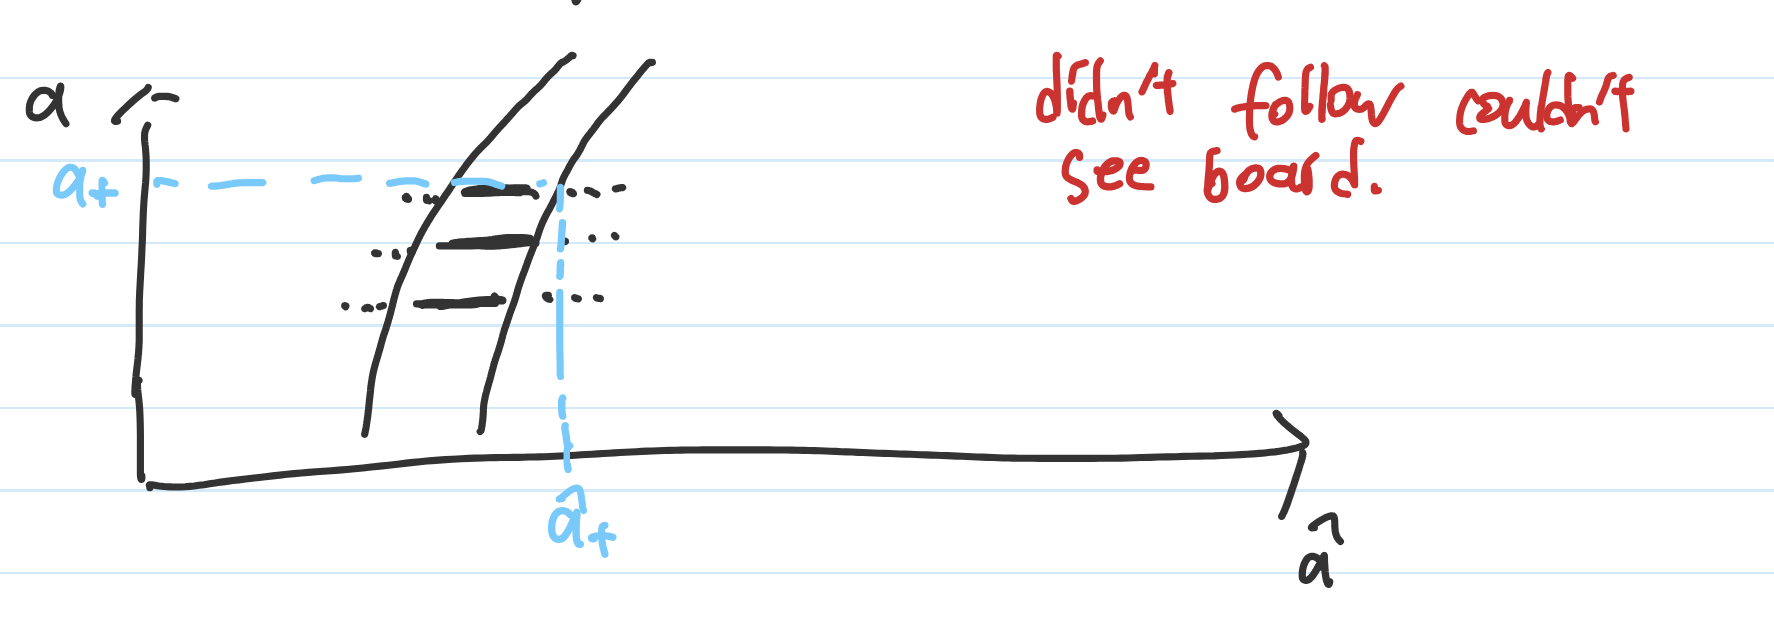
\includegraphics[width = 0.6\linewidth]{Images/lec11-fit-connect.png}\\
    \item $P(a_{-} \leq a \leq a_{+}) = 0.90$, Coverage = fraction of time your prescription for the estimator interval contains the true value a.
    \item Basically we find out/ choose $\hat{a_{-}}$ and $\hat{a_{+}}$ such that 90\% of the time, the true a is in our interval (which corresponds to $a_{-}$ and $a_{+}$).
    \item The Bias of all this is we can really pick intervals however we want.\\
          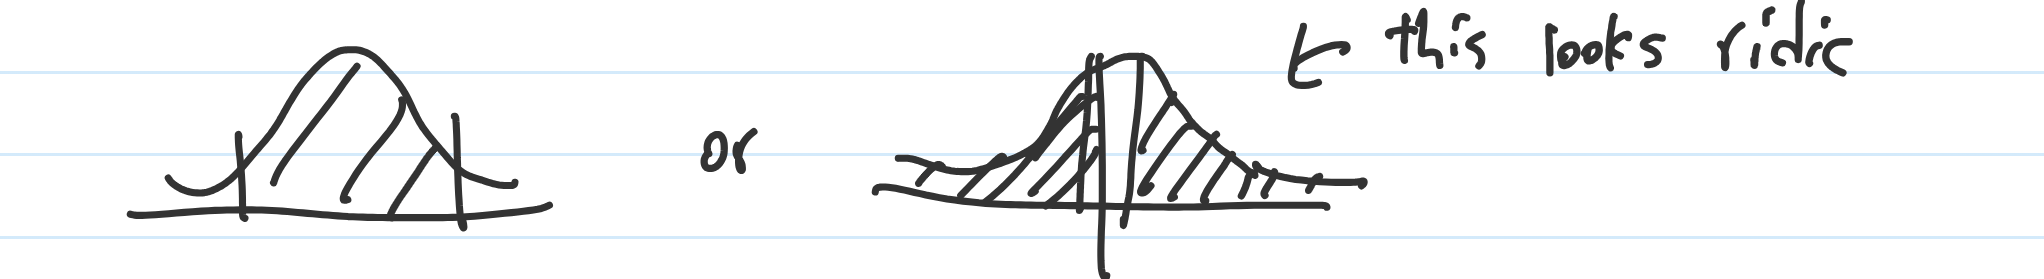
\includegraphics[width = 0.6\linewidth]{Images/lec11-biased-intervals.png}\\
          \divider
    \item Typical Usage of Least Squares (LS):
          \begin{enumerate}
              \item $x_i$, $y_i$, with known $\sigma_{x}$, known $\sigma_{y}$ for $y_i$ \\
                    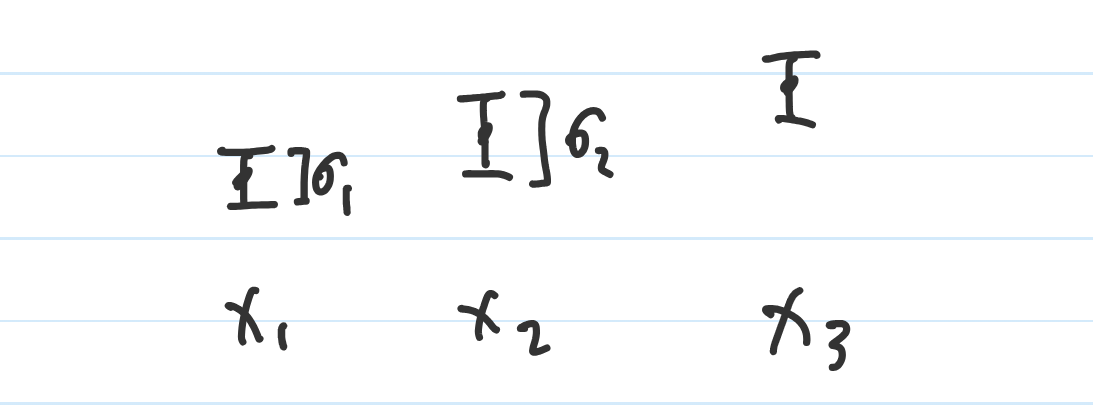
\includegraphics[width = 0.4 \linewidth]{Images/lec11-points.png} \\
                    If $y_{i}$s are measured by detector, we can figure out $\sigma_{i}$ by analyzing the detector. \\
              \item Histograms: i.e. measure x on a coord, can have resolution effects etc, where $y = $ statistics of \# of events of same x. \\
                    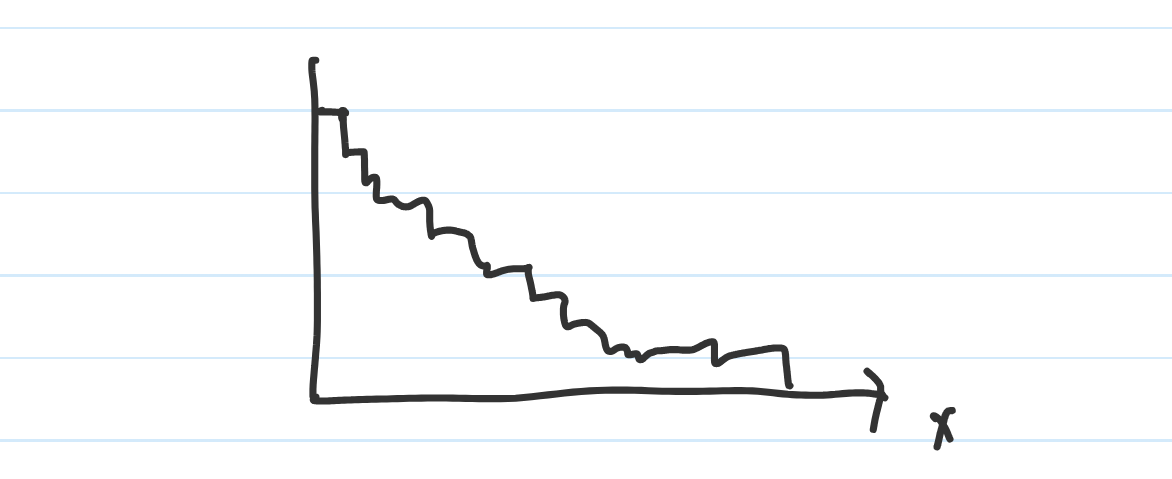
\includegraphics[width = 0.4 \linewidth]{Images/lec11-histogram.png}\\
                    Say resolution has: \\
                    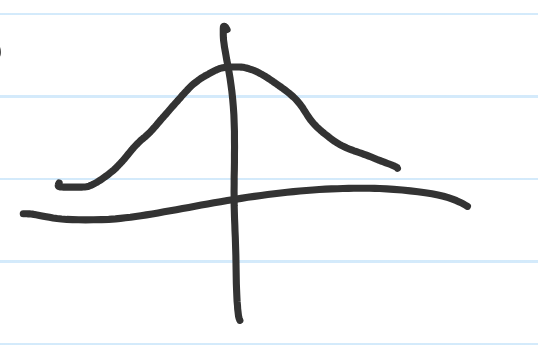
\includegraphics[width = 0.4 \linewidth]{Images/lec11-resolution.png}\\
                    so what you see is actually a convolution of true distribution with resolution function.\\
                    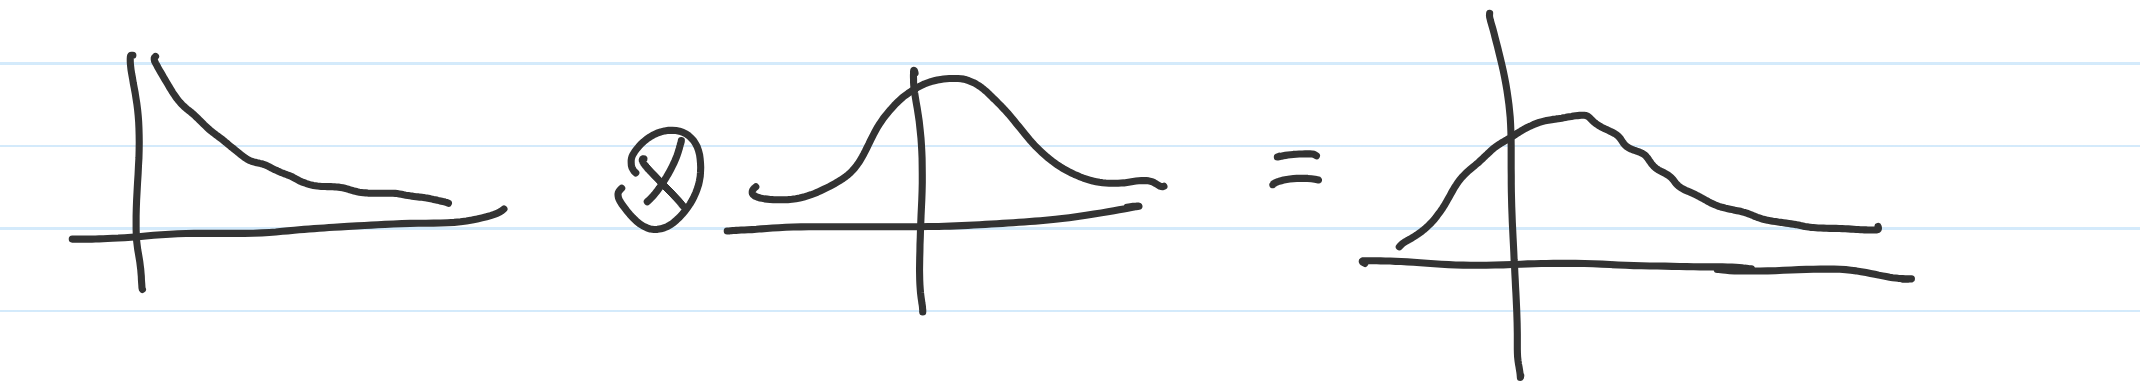
\includegraphics[width = 0.4 \linewidth]{Images/lec11-convolution.png}\\
                    So fit should actually be an exponential $\circledast$ gaussian in this case.\\
                    \[ \chi^2 = \sum_i \frac{(n_i - f_i(\theta))^2}{\sigma_{i}^2} \]
                    say we expect Poisson
                    \[ \sigma_i^2 = n_i \]
                    Data weighted by $n_i$.
                    \[ \text{Neyman } \chi^2 \equiv \sum_i \frac{(n_i - f_i(\theta))^2}{n_i} \]
                    which is a modified least squares. \\
                    Or is sensible to say the expected entries are given by our Model\\
                    $\Rightarrow$ We should use $f_i(\vec{\theta})$ as the mean.
                    $\Rightarrow$
                    \[ \text{Pearson } \chi^2 \equiv \sum_i \frac{(n_i - f_i(\theta))^2}{f_i(\theta)} \]
                    For Neyman $\chi^2$, if a bin is empty, $n_i = 0$ then it blows up. Both Neyman and Pearson are biased oppositely. One could use Neyman and Pearson together but is it worth the effort?
          \end{enumerate}
\end{itemize}

